
\documentclass{sig-alternate}
  \pdfpagewidth=8.5truein
  \pdfpageheight=11truein

\usepackage{cite}
\usepackage{color}
\usepackage{courier}
\usepackage{listings}
\usepackage{url}
%\usepackage{balance} % Add this back in. Probably needed during camera ready.
%\usepackage{listings} % Not sure this does anything here
\usepackage{tikz} % Need for all tikz material
\usetikzlibrary{shapes,arrows, positioning} %  Need for all tikz material
%\usepackage{balance}

\usepackage{times} % Used for formatting formatting url footnotes
\urlstyle{same} % Used for formatting formatting url footnotes
\usepackage{caption} % Used for formatting formatting url footnotes
\usepackage{graphicx}
\usepackage{subcaption}

\newif\ifisnopii
\isnopiifalse % change to false to remove personally identifiable information (pii)


\lstset{ %
language=,                % Make language be nothing
basicstyle=\footnotesize,       % the size of the fonts that are used for the code
numbers=left,                   % where to put the line-numbers; possible values are (none, left, right)
numberstyle=\tiny\color{gray}, % the style that is used for the line-numbers
stepnumber=1,                   % the step between two line-numbers. If it is 1 each line will be numbered
numbersep=-3pt,                  % how far the line-numbers are from the code
backgroundcolor=\color{white},  % choose the background color. You must add \usepackage{color}
showspaces=false,               % show spaces adding particular underscores
showstringspaces=false,         % underline spaces within strings
showtabs=false,                 % show tabs within strings adding particular underscores
%frame=single,           % adds a frame around the code
tabsize=2,          % sets default tabsize to 2 spaces
captionpos=b,           % sets the caption-position to bottom
breaklines=true,        % sets automatic line breaking
breakatwhitespace=false,    % sets if automatic breaks should only happen at whitespace
escapeinside={\%*}{*)}          % if you want to add a comment within your code
}

\setlength{\abovecaptionskip}{6pt plus 3pt minus 2pt} % Space over captions
%\setlength{\belowcaptionskip}{6pt plus 3pt minus 2pt} % Space under captions







\newcommand{\todo}[1]{\textcolor{cyan}{\textbf{[#1]}}}
\newcommand{\sam}[1]{\textcolor{red}{{\it [Sam says: #1]}}}
\newcommand{\dan}[1]{\textcolor{blue}{{\it [Dan says: #1]}}}


\begin{document}
%
% --- Author Metadata here ---
\conferenceinfo{SAC'15}{April 13-17, 2015, Salamanca, Spain.}
\CopyrightYear{2015} % Allows default copyright year (2002) to be over-ridden - IF NEED BE.
\crdata{X-XXXXX-XX-X/XX/XX}  % Allows default copyright data (X-XXXXX-XX-X/XX/XX) to be over-ridden.
% --- End of Author Metadata ---

\title{Concolic Threat Analysis: Detecting Repackaged Android Applications}
\numberofauthors{1} %  in this sample file, there are a *total*
% of EIGHT authors. SIX appear on the 'first-page' (for formatting
% reasons) and the remaining two appear in the \additionalauthors section.
%
\ifisnopii % turn on/off pii
\author{
%
% 1st. author
\alignauthor
Daniel E. Krutz, Samuel A. Malachowsky, Patrick J. McAfee, and Justin M. Peterson\\ 	
	\affaddr{Software Engineering Department}\\
       \affaddr{Rochester Institute of Technology}\\
       \affaddr{1 Lomb Memorial Drive}\\
       \affaddr{Rochester, NY 14623} \\
       \email{\{dxkvse, samvse, pjm4439, jmp3833\}@rit.edu}
} % Must not be a space above this
\else % turn on/off pii
\author{
\alignauthor
XXX X XXX\\
       \affaddr{xxxxx}\\
       \affaddr{xxxx, xx, xxx}\\
       \email{xxxxx@xxx.xxx}
}
\fi % end turn on/off pii

\maketitle
\begin{abstract}

The Android platform has emerged as a market leader largely due to its flexibility, ability to run on a diverse set of hardware, and its flexibility in allowing users to freely install applications from a wide variety of sources. Unfortunately, a significant portion of Android applications (\emph{apps}) are repackaged versions of legitimate applications, often containing malware. Excepting small variations in the source code, they often precisely mimic their legitimate counterparts, making detection of these malicious applications very difficult for end users, researchers, and app store protection systems.

In this paper, we propose a new process called Concolic Threat Analysis (CTA). This static analysis process will form a powerful Android repackaging detection technique as it only traverses the functional aspects of the application, and is not affected by the syntax of the application's code. Furthermore, we demonstrate how concolic analysis can be used to detect repackaged Android applications (potentially identifying malware threats) and lay the foundation for future research.
\end{abstract}


% I think this is the most appropriate
%\ccsdesc[500]{Security and privacy~Software and application security}
\category{D.4.6}{Operating Systems}Security and Protection;
%They are here: http://www.acm.org/about/class/ccs98-html

%\terms{xxx, xxx, xxx}
\keywords{Android, Malware, Repackaged Applications}



% Add in categories and keywords


\section{Introduction}
% Introduce the problem
% What do I plan on accomplishing
%	How is the work I am doing important
% H


% Potential tools
% Really outline how I will do the study and how it will be successful
%

%\sam{Dan, there is a code snip after this that you can use in-line in the paper to make the parts anonymous.  The switch is right after the usepackages and is currently set to anonymous}
%\ifisnopii the non-anonymous text\else the anonymous text or XXXX\fi

The Android platform has gained widespread popularity largely due to its flexibly: its open source nature, the ability to download apps from a wide range of sources, and its ability to operate on a wide variety of mobile devices. Unfortunately, this openness can also lead to severe security vulnerabilities. Anyone may extract the source code of the application file~(\emph{.apk}), giving malicious developers the ability to download a legitimate version of an app, view its source code using a simple reverse engineering process (or a tool such as dex2jar\footnote{https://code.google.com/p/dex2jar/}), inject malicious code, and then upload the visually similar modified version for users to unwittingly download~\cite{Gibler_adrob:examining}. While GooglePlay, the largest Android app store, employs various protection techniques against these repackaged apps~\cite{bouncer_url1}, 3rd party app sites such as AppksAPK\footnote{http://www.appsapk.com/} and F-Droid\footnote{https://f-droid.org/} offer essentially no protection. Previous research shows that about 5\%-13\% of apps in third party markets have been repackaged~\cite{Zhou:2012:DRS:2133601.2133640}, and a recent study~\cite{Zhou:2012:DAM:2310656.2310710} found that 86\% of malware samples were re-packaged Android apps, which is an indication of the formidability of this attack method.

Repackaged Android apps are often very difficult for users to discover, as they may appear to be visually and functionally equivalent to the legitimate app, and may be used for years with no sign of malicious functionality. Researchers often have a hard time detecting the difference between these apps since they are so functionally similar, often with very little source code variation between legitimate and malicious apps. Current techniques for detecting repackaged Android apps include those based on dependency graphs~\cite{Chen:2014:AAS:2568225.2568286}, fuzzy hash matching~\cite{Zhou:2012:DRS:2133601.2133640}, and user interface based approaches~\cite{Zhang:2014:VTO:2627393.2627395}.



% Show example of repackaged application and the malicious source code?
In the following section, we propose a new technique for detecting repackaged Android apps called Concolic Threat Analysis (CTA). A concolic analysis based approach such as this has the advantage of only examining the functional nature of the app and is not affected by common obfuscation attempts, such as altering of naming conventions, insertion of whitespace, or other syntactical changes~\cite{krutz2013cccd}.

% Good site for describing malicious copy of coin pirates
% http://blog.trendmicro.com/trendlabs-security-intelligence/trojanized-android-app-checks-for-keywords-in-sms-messages/


% Describe repackaged Applications and why they are a problem


% Describe what they are
% Why are they a problem
% Show a brief example of how an application can be repackaged
%	Think about using coin pirate as an example

% Describe how applications signed by different developers are an indication of a repackaged application

\begin{figure*}[t]

\begin{center}
% Define block styles
\tikzstyle{line} = [draw, -latex']

\tikzstyle{action} = [draw=none, ellipse,fill=white!20, node distance=1.6cm, minimum height=2em, align=center]
\tikzstyle{block} = [rectangle, draw, fill=white!20, node distance=1.6cm, text width=5em, text centered, rounded corners, minimum height=4em, align=center]
\begin{tikzpicture}[node distance = 2.0cm, auto]

    % Place nodes
	\node [block] (App1) {App \#1};
	\node [action, below of=App1] (Act1) {Similar Size\\Same Category\\Different Key};
	\node [block, below of=Act1] (App2) {App \#2};
	
	\node [block, right=2.0cm of App1] (Source1) {Source Code};
	\node [block, right=2.0cm of App2] (Source2) {Source Code};
	
	\node [block, right=2.0cm of Source1] (Concolic1) {Concolic Output};
	\node [block, right=2.0cm of Source2] (Concolic2) {Concolic Output};
	
	\node [action, below right=0.5cm of Concolic1] (Distance) {Levenshtein\\Distance\\Metric};
	\node [block, right=0.3cm of Distance] (Results) {Similarity Score};
	
	\draw[->] [thick] (App1) to  node {Decompile} (Source1);
	\draw[->] [thick] (App2) to  node {Decompile} (Source2);
	
	\draw[->] [thick] (Source1) to  node {Analysis} (Concolic1);
	\draw[->] [thick] (Source2) to  node {Analysis} (Concolic2);
	
	\draw[->] [thick] (Concolic1) to  node {} (Results);
	\draw[->] [thick] (Concolic2) to  node {} (Results);
\end{tikzpicture}
\caption{Comparision Process to Determine Repackaged App Candidates}
\label{fig:comprocess}
\end{center}
\end{figure*}


%\section{Concolic Analysis}
%\label{sec: conclusion}

% How does concolic analysis work
%	


%Concolic analysis combines concrete and symbolic values in order to traverse all possible paths (up to a given length) of an application. Concolic Analysis is not affected by factors such as naming conventions, syntax and comments. Traditionally, concolic analysis has been used for software testing~\cite{Sen:2005:CCU:1081706.1081750}, code clone detection~\cite{krutz2013cccd} and vulnerability detection~\cite{Chen:2014:CIB:2554850.2554875}. Since concolic analysis is not affected by syntax or comments, identically traversed paths are indications of duplicate functionality, and is therefore functionally equivalent code~\cite{krutz2013cccd,krutz2013code}. Very large amounts of duplicated code in Android applications, which have been signed by different developers, is an indication of a potentially repackaged application. \dan{Not sure if I should saw anything more about CA. I don't in my CCCD tools paper.}




%We show example concolic output in Listing~\ref{lst:concolicoutput}, where constant variable types are represented generically by ``CONST'' while the variable type integer is represented by a generic tag ``SYMINT.'' Though not present above, other variable types are represented in a similar fashion in concolic output such as this. Actual variable names do not appear anywhere in the output and are irrelevant to the concolic analysis technique. We more complete example of concolic analysis and its output may be found on our project website.\todo{Add this data to the website - also add a link to the site as well?}

%\begin{lstlisting}[label=lst:concolicoutput, caption=Example Concolic Output]
%PC#=3
%CONST_3>a_1_SYMINT[2]&&
%CONST_2<=a_1_SYMINT[2]&&
%CONST_1<=a_1_SYMINT[2]
%PC#=2
%CONST_2>a_1_SYMINT[1]&&
%CONST_1<=a_1_SYMINT[1]
%PC#=1
%CONST_1>a_1_SYMINT[2]
%\end{lstlisting}

%\todo{should we show this output here? Maybe compare to sets of identical concolic output }
%\todo{center output, remove lines?}





% Talk about developers signing applications.

% Why will concolic analysis detect duplicate infroatmion.




% Talk about the concolic output very briefly and what is included in it

%\cite{qin2014detecting}

% Show examples from the journal paper?

%\todo{Show how similar malware can be detected as well.}
%\todo{Show a brief example of CA?-- I do not feel I am describing CA well enough here}










% Give a name to this technique
% Find a better title for this
\section{Concolic Threat Analysis (CTA)}
%\label{sec: conclusion}

% Maybe use URL of Java Path Finder is space is an issue? http://babelfish.arc.nasa.gov/trac/jpf/wiki
Concolic analysis combines concrete and symbolic values in order to traverse all possible paths (up to a given length) of an app. Traditionally it has been used for software testing~\cite{Sen:2005:CCU:1081706.1081750}, code clone detection~\cite{krutz2013cccd}, and vulnerability recognition~\cite{Chen:2014:CIB:2554850.2554875}. Since concolic analysis is not affected by syntax or comments, identically traversed paths are indications of duplicate functionality, and therefore functionally equivalent code~\cite{krutz2013cccd,krutz2013code}. These traversed paths are expressed in the form of~\emph{concolic output} which represents the execution path tree and typically displays the utilized path conditions and representative input variables; the precise nature of the output is dependent on the selected concolic analysis tool. Very large amounts of duplicated code in Android apps which have been signed by different developers is an indication of a potentially repackaged app.

Concolic Threat Analysis (CTA) will utilize a process similar to Concolic Code Clone Detection (CCCD), which \ifisnopii we \else was \fi proposed in a previous work~\cite{krutz2013cccd}. CCCD detects duplicate functionality by first performing concolic analysis on the target source code, then separating the output at the method level, and finally comparing methods against each other using a string comparison metric, likely the Levenshtein distance metric. A high similarity score is an indication of redundant functionality, and potentially duplicate or very similar source code. One of the biggest differences between CCCD and our proposed technique is that we will be unable to use CREST\footnote{https://code.google.com/p/crest/} as a concolic analysis engine since it is only compatible with C. We will use another tool such as Java Path Finder (JPF)\footnote{http://babelfish.arc.nasa.gov/trac/jpf/wiki}, jCUTE\footnote{http://osl.cs.illinois.edu/software/jcute/}, or will adapt other existing techniques such as the concolic analysis method developed by Anand~\emph{et al.}~\cite{Anand:2012:ACT:2393596.2393666}. Sample concolic output of JPF and jCUTE are shown in Figure \ref{fig:exampleoutput}.

\begin{figure} [h]
\vspace{2 mm}

\begin{subfigure}[b]{0.48\textwidth}
	\label{fig:JavaPathFinder}
	\begin{lstlisting}
	PC#=3
	CONST_3>a_1_SYMINT[2]&&
	CONST_2<=a_1_SYMINT[2]&&
	CONST_1<=a_1_SYMINT[2]
	PC#=2
	CONST_2>a_1_SYMINT[1]&&
	CONST_1<=a_1_SYMINT[1]
	\end{lstlisting}\caption{Java Path Finder}
\end{subfigure}
\begin{subfigure}[b]{0.48\textwidth}
	\label{fig:jCUTE}
	\begin{lstlisting}
	jwtc.chess.Move: boolean isOO(int)
	jwtc.chess.Move: boolean isOOO(int)
	java.lang.StringBuilder: void <init>()
	Method setOptionExtraOptions value  read
	Method setOptionLogLevel value 3 read 3
	Method setOptionPrintOutput value true
	\end{lstlisting}\caption{jCUTE}
\end{subfigure}
%\end{tabular}
%\dan{I added indents to the code and cleaned things up in this table}
\caption{Example concolic output~\label{fig:exampleoutput}}
\end{figure}

Similar to previous research~\cite{Zhou:2012:DRS:2133601.2133640}, we assume that repackaged apps are of the same type or category as the legitimate version, that the size of the two do not differ substantially (due to the small amount of altered code), and that they have not been signed with the same key (assuming that original keys have not leaked). Only comparing apps of similar size, in the same category, and with different keys will assist in significantly limiting the amount of comparisons that need to be conducted. The process which CTA will use to find repackaged Android applications is shown in is shown in Figure \ref{fig:comprocess}.


As a proof of concept, we built a sample application based on public Android code and a known malware example. This application a was a clone of Android Chess\footnote{https://github.com/jcarolus/android-chess} injected with a common premium SMS exploit\footnote{https://www.webroot.com/shared/pdf/Android-Malware-Exposed.pdf}, focusing on common activities that were not directly tied to the activity model.  Due to the limitations and requirements of jCUTE, the easy-to-implement analysis tool selected for the prototype, Android interactions were mocked out and a wrapper to call specific functions was created.  Running jCUTE on this sample app provided text output that demonstrated the flow of calls to naked functions. We manually compared the concolic output produced when running jCUTE on both the malicious and original versions of the application; a sample is shown in Figure~\ref{fig:diff1}. While both use concolic analysis, the output of jCUTE and JPF are very different in that JPF shows utilized concrete and symbolic values, and jCUTE only displays the traversed method signatures. Because of this, we will likely choose to use JPF for our final implementation.

%The primary tool chosen for this purpose was jCUTE, which we selected since it was easy to implement and produced easily understandable results.
\begin{figure*}[t]
\centering
%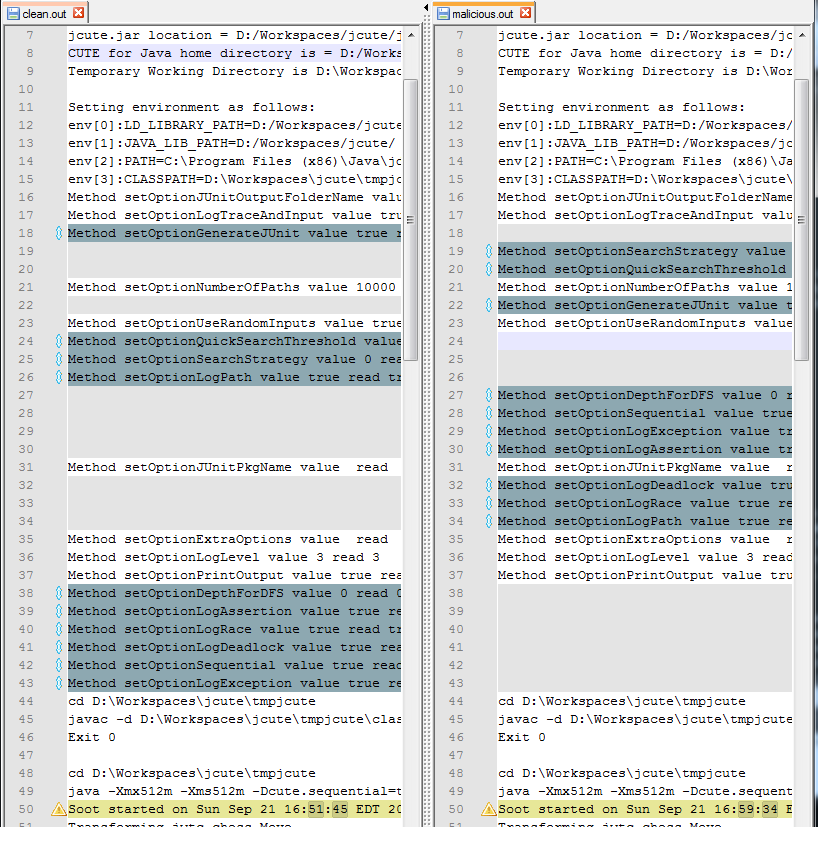
\includegraphics[width=17cm, angle = 0]{images/diff1a.png}
\begin{subfigure}[b]{0.49\textwidth}
	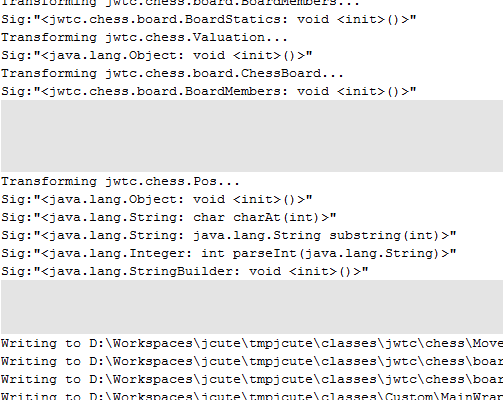
\includegraphics[width=8.5cm, angle = 0]{images/DiffClean2.png}
	\caption{Original}
	\label{fig:original}
\end{subfigure}
\begin{subfigure}[b]{0.49\textwidth}
	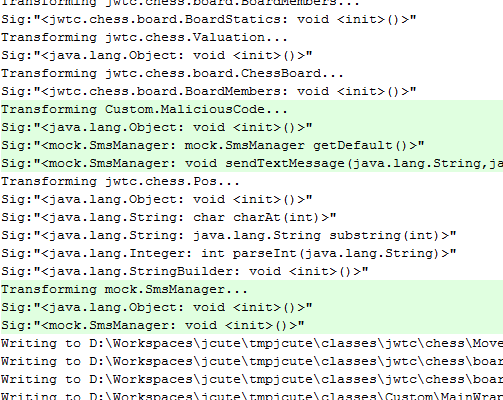
\includegraphics[width=8.5cm, angle = 0]{images/DiffMalicious2.png}
	\caption{Repackaged malicious}
	\label{fig:malicious}
\end{subfigure}
\caption{Diff of concolic output of modified application versions}
\label{fig:diff1}
\end{figure*}

%\sam{left off here}
This~\emph{diff} of the concolic output demonstrates the substantive differences between the two versions of the application and how a concolic based technique can be used to find variations in Android application versions - instances where an application has been repackaged and could be malicious. Complete results, existing project source code, and further project information may be found on our project website\footnote{\ifisnopii \url{http://www.se.rit.edu/~dkrutz/CTA/}\else site removed to keep paper anonymous\fi}.


\section{Future Work \& Conclusion}
\label{sec: conclusion}


% What hurdles do we have to overcome
%	Speed
%	Lots of code snippets - only looking for significant functionality
%		? How do other applications do this
% Only separated at method level
%	Is this a problem?
%	How will it be addressed in the future?

% Will not be able to detect some malware.... IE simple text links.
%


Several barriers must be overcome in this approach; the largest is related to the fact that Android applications lack a main method and only implement parts of the Android SDK API. The absence of a main method makes it very difficult to run existing concolic analysis tools, because main methods are often a requirement~\cite{Anand:2012:ACT:2393596.2393666}. In order to address this issue, we will either alter an existing concolic analysis tool (such as JPF), or employ an approach similar to that of Anand~\emph{et al.}~\cite{Anand:2012:ACT:2393596.2393666}, who use an approach based on concolic testing and event sequences.


% We will also need to devise a way of comparing large numbers of Android applications to detect repackaged applications.

% Put in a filler between these two segments


%The next phase of our research will be to create a more robust detection tool, conducting a more widespread analysis on the capabilities of concolic analysis in detecting repackaged Android applications. The initial step will be to create a concolic analysis based tool to generate the necessary output for comparison. We will likely follow a process presented by Anand~\emph{et al.}~\cite{Anand:2012:ACT:2393596.2393666}, but are exploring other possibilities as well, such as modifying JPF. \sam{This needs rework.  Should we say that we are continuing development of CTA as a tool rather than just a process?}\dan{Lets talk, I am not sure what you mean}
%\sam{I took out an entire paragraph, as it seemed like a repeat of the one before it.}

% Should JPF be cited? ~\cite{Visser:2004:TIG:1013886.1007526}


% List some of the challenges of making the tool
%   No main methods in Android applications



% Look and see if there are other resources available
%


Once the tool has been completed, we will conduct our analysis in several phases. First, we will evaluate our tool in a controlled environment comparing known repackaged applications (identified by sources such as Conagio Mobile\footnote{http://contagiominidump.blogspot.com} and the Malware Genome Project\footnote{http://www.malgenomeproject.org}) to their legitimate counterparts. Next, we will compare non-repackaged applications in order to ensure that our technique exceeds acceptable levels of precision and recall. Finally, we will examine Android applications from sources such as GooglePlay and AppsAPK to discover repackaged applications which may have been previously undiscovered, comparing our findings to previously proposed techniques for detecting repackaged applications~\cite{Chen:2014:AAS:2568225.2568286, Zhou:2012:DRS:2133601.2133640,Zhang:2014:VTO:2627393.2627395}.

In this work, we outlined the problem of repackaged Android applications and described a possible solution for detecting them using concolic analysis. We also demonstrated a protoytpe which was able to detect malicious code in a small, controlled environment. Finally, we described our future work and discussed some challenges which will need to be overcome in the next phases of development.


% More robust testing of applications
% Will do a larger study


\bibliographystyle{abbrv} % Check on this
\bibliography{Repackaged_Android}

% that's all folks
\end{document}




%%%% Todo
% Make sure entire formatting is correct
% Fix the author list at the top of the document
% Add in categories and keywords section
% Do labels go on top or bottom?
%	I think tables and figures go on bottom
% Find name of our tool
% Create website to share our results - http://www.se.rit.edu/~dkrutz/RAA/
%   Create a GH repo to tie data in



% Notes
% SACS - 9/12 -  2 pgs notify: 11/17
%	http://www.acm.org/conferences/sac/sac2014/Author-kit-2014.pdf
% ICSE 11/21 4 pgs notify:1/21
%	http://2015.icse-conferences.org/call-dates/call-for-contributions/nier-2015


% 2 pages, a third is an extra $80 cost

% Thoughts
%   If we cannot find a good example of malware, we can create our own example
%

% Possible links
%   http://contagiominidump.blogspot.com/2014/05/android-fake-av-se-cure-mobieav.html
%   http://blogs.360.cn/360mobile/2014/04/02/analysis_of_oldboot_b_en/

% http://blog.andrototal.org/post/89637972097/another-android-trojan-scheme-using-google-cloud
%       May be a good way of showing that all of the similar malware copies can be detected


